%!TEX root = sui14.tex
\section{IR for head orientation-based targeting}
In this section, we present our hardware platform (IR targeting) and interaction model (head-orientation based) that we will use throughout our iterative designs.

\subsection{Hardware}
%A central hypothesis of this paper is that the area cursor paradigm~\cite{kabbash1995prince} is well matched to head orientation selection. Head orientation input is imprecise because it does not capture eye movement and has to rely on a low-bandwidth muscle group. Therefore, point selection techniques like laser pointers are not appropriate. 

We hypothesize that infrared (IR) emitters are a good technology match for head orientation selection, since they emit light within a given angle, resulting in a cone in front of the emitter where the light is visible. IR LEDs with many different beam angles are commercially available. We augment Google Glass with a 940nm 5mm IR emitter with $10^\circ$ beam angle (OSRAM SFH 4545). The emitter is controlled by an additional microcontroller which communicates with Google Glass through Bluetooth radio, since Glass does not directly support hardware modification (see Figure~\ref{fig:glass}). Target devices use Vishay TSOP38238 IR receivers. Data is encoded using standard IR remote protocols at 38.0kHz.

IR signals are used for initial line-of-sight targeting; subsequently, we use bi-directions wireless communication to send information such as target IDs and signal strength from targets to back to Glass. We have chosen the commercial off-the-shelf ZigBee implementation (XBee based on 802.15.4 radio) for this purpose (see Figure~\ref{fig:architecture}). This architecture was mostly chosen for reasons of expediency and we do not claim optimality for prototyping decisions. Future head-mounted devices could clearly integrate IR emitters; other wireless techniques (WiFi, Bluetooth) can also be used.

% The IR emitter is the one from OSRAM Opto Semiconductors Inc with manufacturer part number SFH 4545. From the datasheet, it has a view angle of $10^\circ$. Part of the reason we have chosen it is because the radiant intensity can quite high if we provide it with sufficient current flow (550mW/sr @ 100mA). We can then easily adjust it using a resistor to satisfy different demands. 
% % transmitter webpage: http://www.digikey.com/product-search/en?x=0&y=0&lang=en&site=us&KeyWords=475-2919-ND
% For the IR receiver, we use 38.0kHz IR Receiver Modules from Vishay Semiconductor Opto Division (manufacturer part number TSOP38238). 
% % receiver webpage http://www.digikey.com/product-detail/en/TSOP38238/751-1227-ND/1681362
% In order to read the IR intensity, we integrates another IR light-to-voltage converter from AMS-TAOS USA Inc (manufacturer part number TSL267-LF) which is pretty sensitive to IR irradiance. 
% % http://www.digikey.com/product-detail/en/TSL267-LF/TSL267-LF-ND/3095052



%% \ben{no mention of target hardware yet. I have checked in an image of the targets ``targets.JPG'' in case we need.}

%For the IR receiver, we use 38.0kHz IR Receiver Modules from Vishay Semiconductor Opto Division (manufacturer part number TSOP38238). 
% receiver webpage http://www.digikey.com/product-detail/en/TSOP38238/751-1227-ND/1681362
%In order to read the IR intensity, we integrates another IR light-to-voltage converter from AMS-TAOS USA Inc (manufacturer part number TSL267-LF) which is pretty sensitive to IR irradiance. 
% % http://www.digikey.com/product-detail/en/TSL267-LF/TSL267-LF-ND/3095052

\begin{figure}[t]
\centering
\includegraphics[width=0.95\columnwidth]{figures/GlassWithArduino.jpg}
\caption{Our Glass hardware: Google Glass augmented with a repositionable IR holder, and an additional microcontroller that communicates with Google Glass and controls IR emitter.}
\label{fig:glass}
\end{figure}

\begin{figure}[t]
\centering
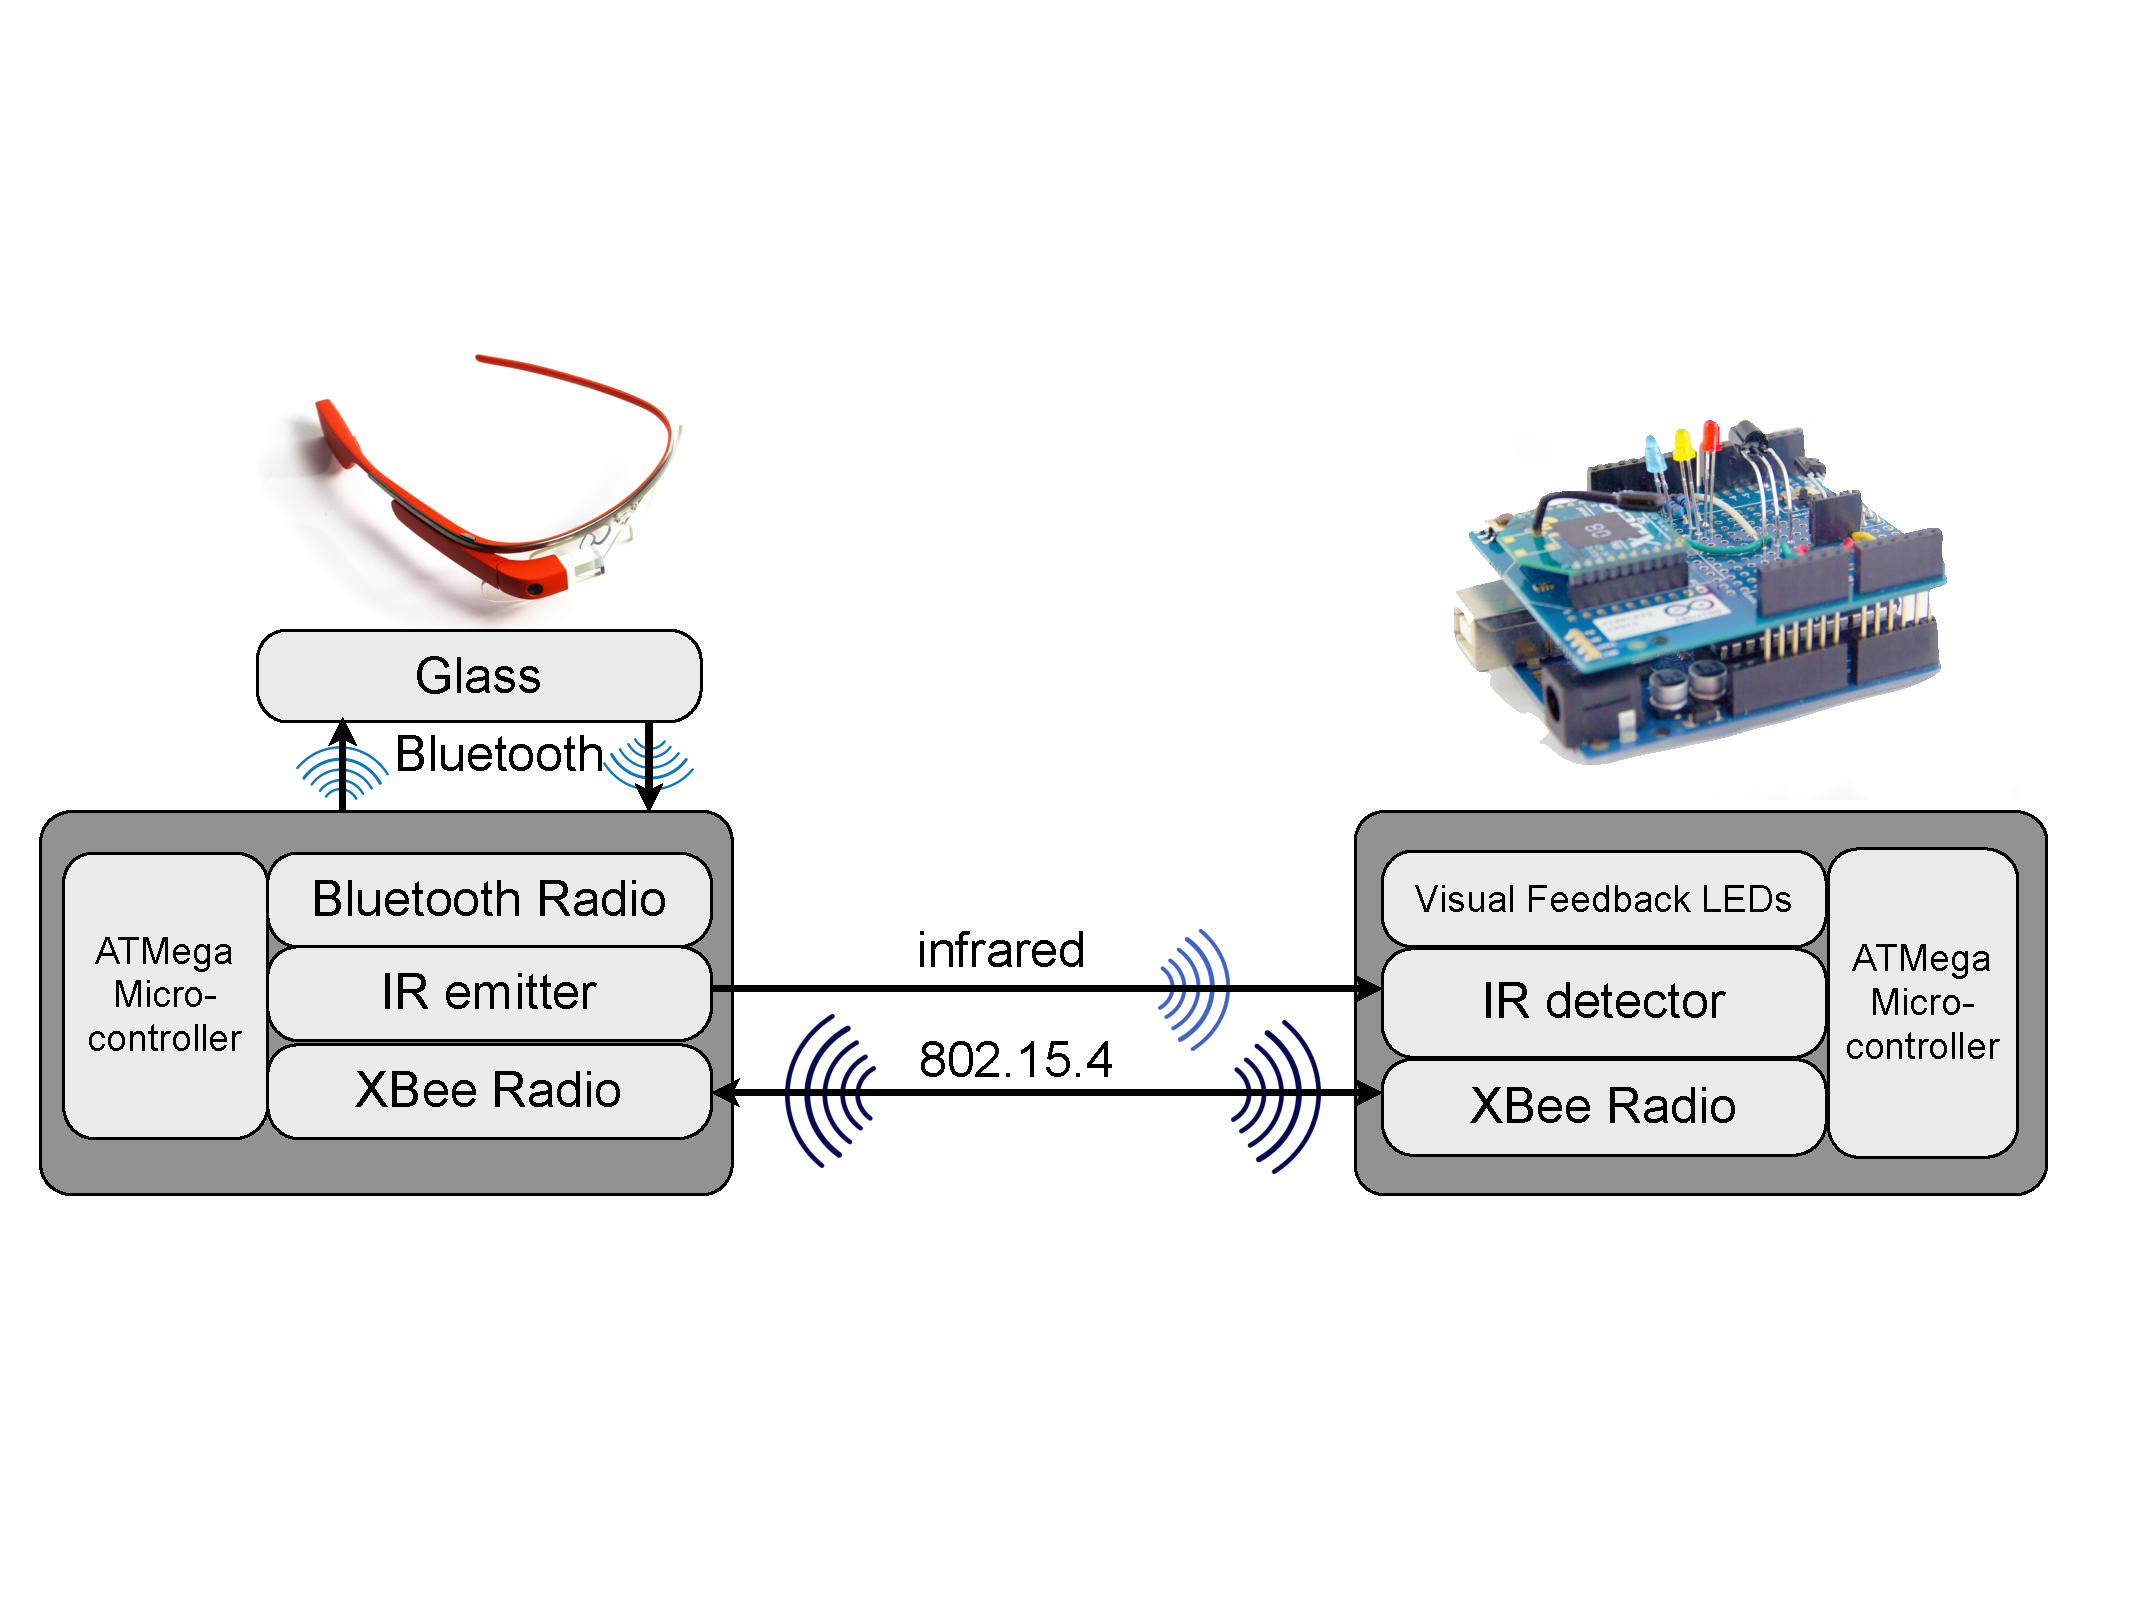
\includegraphics[width=0.95\columnwidth]{figures/architecture_new}
\caption{Our System architecture diagram. The selection is initiated through infrared but confirmed over 802.15.4.}
\label{fig:architecture}
\end{figure}


\subsection{Interaction Model}
From the user's perspective, interaction with \systemname proceeds in two stages (Figure~\ref{fig:interaction}): 


{\bf Scan:} The user first scans the environment to locate the position of the target. During this stage, Glass constantly sends out IR signals, and  targets offer immediate visual feedback when they receive a signal. The user confirms his desire to connect to a target by tapping on the Glass touchpad. Glass collects the responses from targets that have received IR reception through the backchannel of XBee. If there is only one single target in IR range, it is automatically selected. However, in a dense environment where multiple targets are within range, the user needs refine his selection.


{\bf Refine:} When disambiguation is needed, the user must make an explicit selection among the targets within their view range. We have designed multiple refinement mechanisms -- all of which enable the user to select one from a subset of targets. The user confirms the current selection with a tap. Since the purpose of this stage is to disambiguate among potential targets, we will also use {\em disambiguation} to refer to this stage. Finally, a tap confirms a decision.


\begin{figure}[t!]
\centering
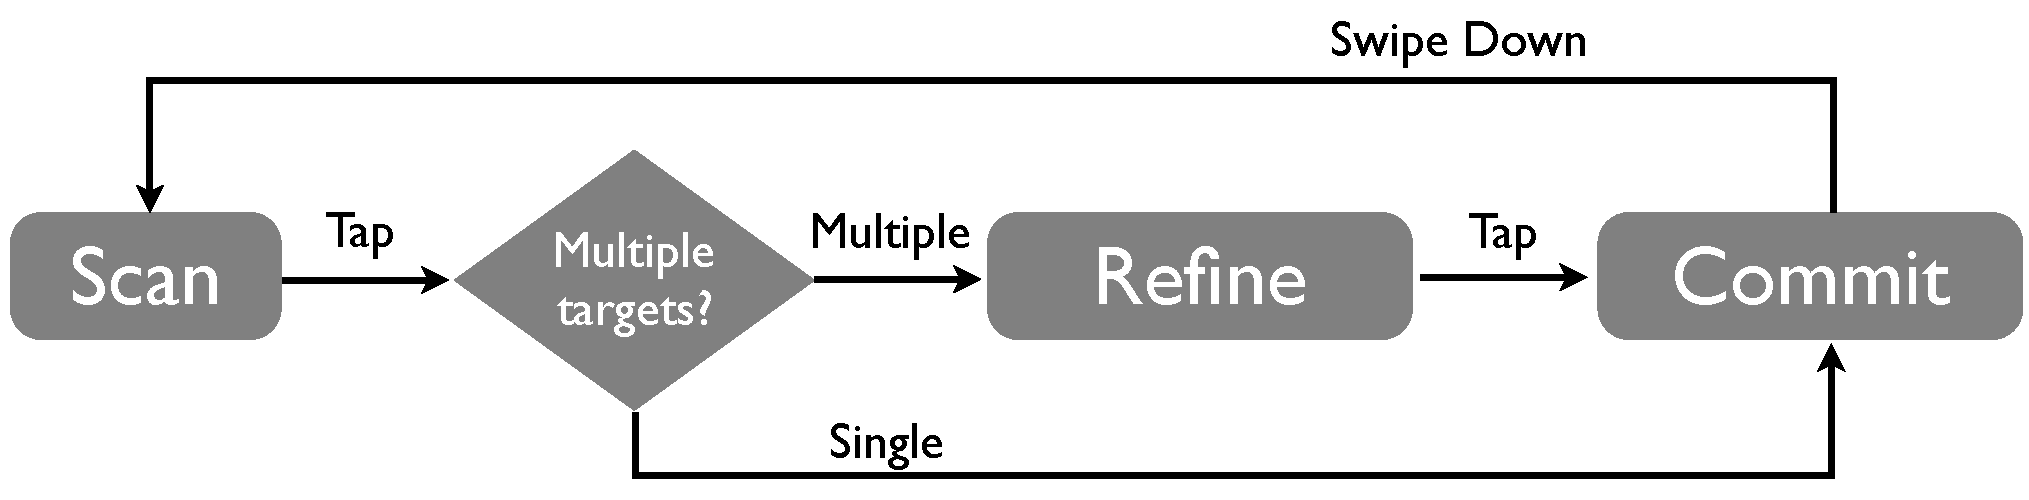
\includegraphics[width=\columnwidth]{figures/interactionModel2.pdf}
\caption{{\em scan} and {\em refine} -- two main stages during the interaction with HOBS. For completeness, we have also added the final state of {\em commit}.} 
\label{fig:interaction}
\end{figure}

The overall target acquisition time thus depends on scan and refine times, the probability that refinement is needed, and the time to commit an action (tap):
\begin{equation}
t_{total}=t_{scan}+P(refine)*t_{refine}+t_{commit}
\label{eq:time}
\end{equation}

In the following sections, we describe our iterative design and evaluation process to minimize the overall target selection time.

%%% Local Variables: 
%%% mode: latex
%%% TeX-master: "uist14"
%%% End: 
